% First release on June 21, 2010
% Modified on Dec 12, 2017 by XSK

\documentclass[twoside,twocolumn]{article}
% \documentclass[twoside,twocolumn]{ctexart}

\usepackage{CJKutf8}	% encode for Chinese
\usepackage{fitee}


%\usepackage[colorlinks, breaklinks = true]{hyperref}		% for pdflatex
\usepackage[hidelinks, breaklinks = true]{hyperref}  % for DVI to PDF latex
\hypersetup{CJKbookmarks=true}

\addto{\captionsenglish}{%
  \renewcommand{\figurename}{图}
  \renewcommand{\tablename}{表}
}
\usepackage{ctex}
% \usepackage{epstopdf}


\begin{document}
\begin{CJK}{UTF8}{song}	% all Chinese should be enclosed between the commands

%% article title
\title{\LaTeX{} 排版技巧总结}

%% when all authors provide emails, no $\dagger$
\author{{\kaishu 翟自洋}}%
\author{\kaishu 张欣欣}
\affil{浙大学报(英文版)编辑部, 浙江大学出版社, 杭州 $310027$, 中国}

\shortauthor{Zhai and Zhang}	% one author: only Zhai; two authors: Zhai and Hu; three authors: Zhai et al.

\authmark{}

%% Only 1 affiliations
%\author{Wen-fei WANG}
%\author{Rong XIONG$^{\dagger\ddagger}$}
%\author{Jian CHU}
%\affil{\it\footnotesize State Key Laboratory of Industrial Control Technology, Institute of Cyber-Systems and Control,
%	\authorcr\it\footnotesize Zhejiang University, Hangzhou 310027, China}

% for authors, use \authorcr to begin with a new line, e.g., \author[2]{\authorcr Xian-liang HU}
% for the affiliation, use \authorcr\Affilfont\it to begin with a new line, e.g.,
%\affil[1]{Editorial Office of Journal of Zhejiang University SCIENCE,
%\authorcr\Affilfont\it Hangzhou 310027, China}

\corremailA{jzus\_zzy@zju.edu.cn}
\corremailB{xlhu@zju.edu.cn}
%\corremailC{abc@zju.edu.cn}
%\corremailD{ABC@zju.edu.cn}
\emailmark{}	% when all authors provide emails, no \dagger


% abbrev. of month: Jan. Feb. Mar. Apr. May June July Aug. Sept. Oct. Nov. Dec.


\abstract{本文档介绍了《浙大学报(英文版)》\LaTeX{} 模板的使用方法, 也总结了 \LaTeX{} 排版时所需的技巧.}

% separate by semicolons



%\inpress	% uncomment this command if use "in press"

\publishyear{2018}
\vol{19}
\issue{1}
\pagestart{1}
\pageend{5}

%% when no funding, the following line should be removed, no period at last


%\conf{A preliminary version of this paper has been presented at ??? Conference, date}
%\esm{Electronic supplementary materials: The online version of this article (http://dx/doi.org/10.1631/jzus.C1000000) contains supplementary materials, which are available to authorized users}
\orcid{}	% corresponding author, or first author
\articleType{}
%\articleType can be `Science Letters:', `Review:', `Comment:', etc.
%Leave blank for research article.


\maketitle



\section{初步编译 \LaTeX{}} \label{sec:introduction}


\begin{figure*}[!t]\small
\centering
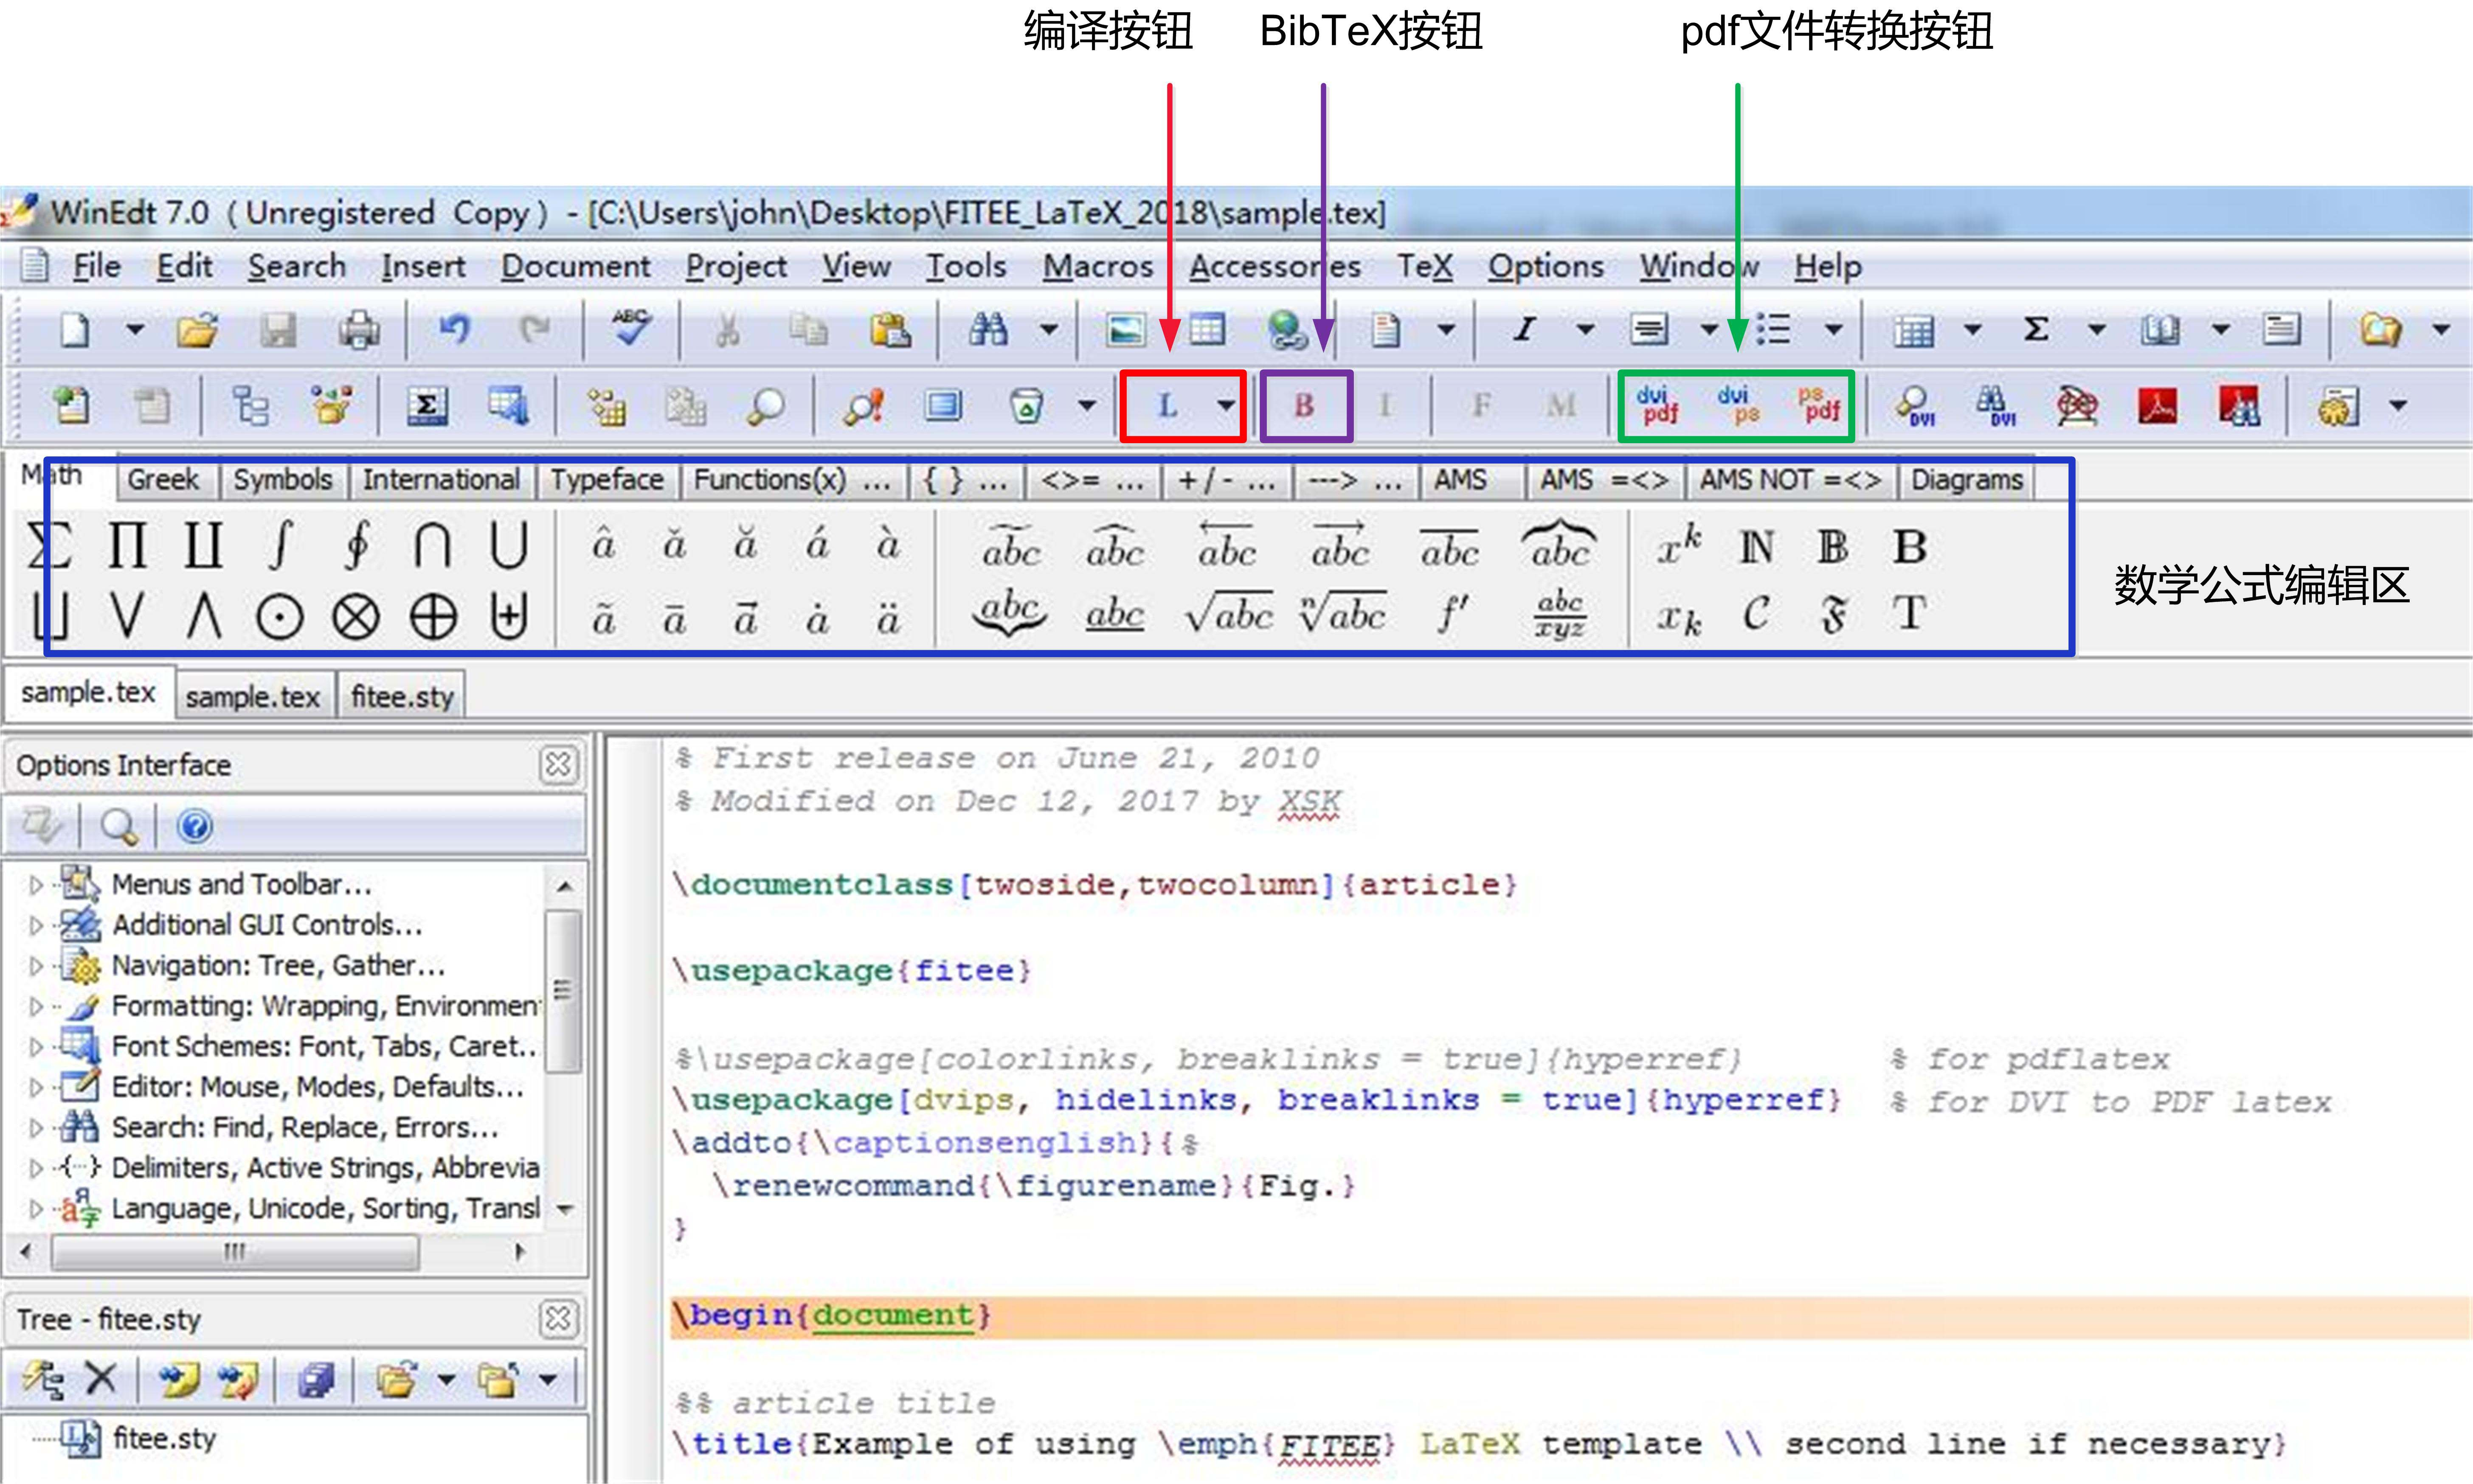
\includegraphics[width = 16.4cm]{latexSum/desktop2.jpg}
\caption{WinEdt 界面示意}
\label{fig:ui}
\end{figure*}

\LaTeX{} 是一种文字排版系统. 相较于 MS-Word, 使用 \LaTeX{} 能排版出更美观的科技论文. 
虽然 \LaTeX{} 能够跨平台使用,《学报》编辑部推荐 Windows 用户使用 CTeX 套件排版, 以便交流. 
CTeX 套件的下载地址为: 
\url{http://www.ctex.org/CTeXDownload}

安装 CTeX 套件后, 即可使用其集成的 WinEdt 编辑器浏览与编辑 \LaTeX{} 文件. 
WinEdt 的主要操作界面如图 \ref{fig:ui} 所示, 其中用不同颜色的矩形框标示出各个主要功能的按钮. 以下, 
针对编辑部网站提供的 \LaTeX{} 模板文件( \url{http://www.jzus.zju.edu.cn/download/FITEE_LaTex_template.zip}), 
介绍 \LaTeX{} 文件的编译过程. 

模板文件夹中包含的主要文件如表~\ref{tab:mainFiles} 所示. 使用 WinEdt 可以直接打开 sample.tex 文件, 
浏览/编辑文件内容(图~\ref{fig:ui}). 文件的编译过程如下: 
\begin{itemize}
  \item 点击图~\ref{fig:ui} 中所示的 \LaTeX{} 编译按钮, 利用 .tex 文件、插图、模板文件生成 .dvi 文件;
  \item 点击图~\ref{fig:ui} 中 pdf 文件转换处的 dvips 按钮, 利用上一步生成的 .dvi 文件生成 .ps 文件;
  \item 再点击 pspdf 按钮, 利用 .ps 文件生成 .pdf 文件, 从而查看写作/排版效果.
\end{itemize}

至此, \LaTeX{} 文件的编译完成. 
与 MS-Word 相比, 使用 WinEdt 编辑 \LaTeX{} 时虽不能随时观察排版的效果, 
但 \LaTeX{} 的版面基本全由模板文件(fitee.sty)控制, 排版人员所需关心的事项反而较 MS-Word 排版明显要少. 
例如, 无需关注稿件章节标题前后的行距和空行, 无需关注字体及字号. 同时, \LaTeX{} 为纯
文本编辑, 无需担心使用 MS-Word 时常出现的“莫名错误”. 本文档即以 \LaTeX{} 排版完成, 为输入中文, 使用了 ctex 宏包. 

\begin{table}[t]
\centering\footnotesize
\caption{FITEE 模板文件夹主要文件列表}
\label{tab:mainFiles}
\begin{tabular*}{7.9cm}{@{\extracolsep{\fill}}lp{5.5cm}}
	\toprule[0.75pt]
	文件名称          & \multicolumn{1}{c}{描述}       \\ 
	\midrule[0.5pt]
	sample.tex    & \LaTeX{} 文件                  \\
	fitee.sty     & FITEE 模板宏包                    \\
	authblk.sty   & FITEE Author Block 宏包         \\
	bibsample.bib & 参考文献数据示例                     \\
	fitee.bst     & FITEE 参考文献格式文件, 用于设置参考文献的排版格式 \\
	orcid16.eps   & ORCID logo 图片                 \\
	fitee.eps     & FITEE logo 图片                 \\
	uarial.sty    & 无衬线字体文件                      \\ 
	\toprule[0.75pt]
\end{tabular*}
\end{table}



\section{\LaTeX{} 稿件首页的处理} \label{sec:related_work}

虽然 \LaTeX{} 稿件的版式基本全由模板文件(fitee.sty)所确定, 
但在实际处理时, 排版人员需编辑稿件首页, 满足使其期刊要求. 
表~\ref{tab:1stPage} 总结出了有关稿件首页信息的关键代码. 
排版人员需针对期刊要求, 逐一修改/确认相关代码. 


\section{插图}
对于 \LaTeX{} 稿件, 编辑部一般要求作者提供 .eps 格式的图片. 
初排时, 排版人员应按照排版手册的要求, 认真修改图片. 在 \LaTeX{}
文件中, 使用如下代码插入图片: 

\begin{table}[!h]
\centering\footnotesize
\caption{插图代码示例}
\label{tab:insertFig}
\begin{tabular*}{7.9cm}{@{}rl}
\toprule[0.75pt]
1. & \textbackslash begin\{figure\}[htbp]\\
2. & \quad\ \textbackslash centering \textbackslash small\\
3. & \quad\ \textbackslash includegraphics[width = 5cm]\{figureSample.eps\}\\
4. & \quad\ \textbackslash caption\{不同编译选项选择方式\}\\
5. & \quad\ \textbackslash label\{fig:pdflatex\}\\
7. & \quad\ \textbackslash begin\{minipage\}[c]\{7.9cm\} \\
8. & \quad\quad\quad \textbackslash vspace\{1.5pt\} \\
9. & \quad\quad\quad \ This figure shows that $\ldots$ (图注文字)\\
10. & \quad\ \textbackslash end\{minipage\} \\
11. & \textbackslash end\{figure\}\\
\bottomrule[0.75pt]
\end{tabular*}
\end{table}

\noindent 插图代码说明: 

1.~第一行代码方括号中参数‘htbp’决定了图片被插入的位置: 

  h: 将图形放在正文中给出该图形的地方;

  t: 将图形放置在页面的顶部;

  b: 将图形放置在页面的底部;

  p: 将图形放置在只允许有浮动对象的页面;

  !: \LaTeX{} 具有默认的页面“审美标准”. 
  在浮动位置选项前加上一个惊叹号‘!’会使 \LaTeX{} 忽略本页面的审美条件.

在方括号中使用上述单个选项(例如 [t])可确定图片在页面中的位置; 使用多个选项的组合(例如~[htb]),
\LaTeX{} 将根据正文自行排布图片. 有关图片排布的更多内容, 请参考
\url{http://www.ctex.org/documents/latex/graphics/node64.html};

2.~图题一律为粗体字. 当图题中有数学公式出现时, 不论其为标量还是矢量, 均应
使用 \$\textbackslash bm\{$\cdot$\}\$ 命令将其改为粗体;

3.~图注常为白体. 在本例中, 使用宽度为 7.9~cm 的 minipage
环境放置图注(第7--10行).


\begin{table*}[!t]
	\centering\footnotesize
	\caption{tex 文件首页代码说明. 其中 1--4 行为导言区, 其他为正文区}
	\label{tab:1stPage}
	\begin{tabular*}{16.4cm}{@{\extracolsep{\fill}}rlp{7.2cm}}
		\toprule[0.75pt]
		序号 & \multicolumn{1}{c}{代码} & \multicolumn{1}{c}{说明}  \\
		\midrule[0.5pt]
		1 & \textbackslash documentclass[twoside, twocolumn]\{article\}    	
		& 文档类型命令: 使用双面、双栏 article 类型排版 \\
		2 & \textbackslash usepackage\{fitee\}     	
		& 调用 FITEE 模板宏包 \\
		3 & \textbackslash usepackage[dvips, hidelinks, breaklinks = true]\{hyperref\}   	
		& 调用超链接宏包 hyperref, 
		其中参数 dvips 表明使用 LaTeX $\rightarrow$ dvips $\rightarrow$ pspdf 等三步流程生成 pdf 文件供浏览; 该参数可改为 dvipdfmx, 从而使用 LaTeX $\rightarrow$ dvipdf 两步流程生成 pdf 文件(对照图~\ref{fig:ui} 中 pdf 文件转换的三个按钮) \\
		4 & \textbackslash addto \{ $\ldots$ \}	& 定义图题样式, 排版人员一般不必理会 \\
		\midrule[0.5pt]
		5 & \textbackslash begin\{document\}     	
		& 正文开始声明 \\
		6 & \textbackslash title\{Example of $\ldots$\}   	
		& 论文标题 \\
		7 & \textbackslash author[\$\textbackslash dagger\$\$\textbackslash ddagger\$1]\{Zi-yang ZHAI\}     	
		& 作者姓名及标注. 其中方括号内为作者标记信息: 
		当提供邮箱时, 标记 $\dagger$; 作为通讯作者, 标记 $\ddagger$; 
		多个单位时, 利用阿拉伯数字 1, 2, $\ldots$ 标注作者所属单位. 作者名首字母大写, 中国作者名首字母大写且以连字符‘-’分隔名中的多个字, 作者姓所有字母大写\\
		&                   & 注意, 当所有作者均属同一单位时, 删去此行代码中的方括号及方括号中的内容, 采用如下方式标注: \\
		&           &
		\textbackslash author\{Zi-yang ZHAI\$\^{}\textbackslash dagger\$\$\^{}\textbackslash ddagger\$\$\^{}1\$\}\\
		8 & \textbackslash affil[1]\{Editorial $\ldots$\}    	
		& 单位名称. 其中方括号内数字为单位的序号. 当仅有一个单位时, 
		应删去方括号及括号中的数字 \\
		9 & \textbackslash shortauthor\{Zhai and Hu\}  & 稿件页眉处的作者信息. 当稿件有两位作者时, 使用本行代码; 当有三位及以上作者时, 使用 Zhai et al. 的形式\\
		10 & \textbackslash authmark\{\}
		& 作者符号, 排版人员一般不必理会\\
		11 & \textbackslash corremailA\{jzus\textbackslash\_zzy@zju.edu.cn\}
		& 作者 email\\
		12 & \textbackslash emailmark\{\$\textbackslash dagger\$\}
		& 作者 email 前的标识符, 当所有作者均提供 email 时, 删去此行代码花括号之间的内容\\
		13 & \textbackslash dateinfo\{Received Nov.\ 11, 2017; $\ldots$\}
		& 收稿、录稿时间信息\\
		14 & \textbackslash abstract\{This brief sample $\ldots$\}
		& 摘要内容\\
		15 & \textbackslash keywords\{ $\ldots$ \}
		& 关键词\\
		16 & \textbackslash doi\{10.1631/FITEE.1000000\}
		& 稿件 doi, 需改动其最后的七位数字. 例如稿件 ZUSC-D-16-01028 的 doi 为
		10.1631/FITEE.1601028\\
		17 & \textbackslash clc\{TP391\}
		& 稿件中图分类号\\
		18 & \textbackslash support\{Project supported by the National Natural $\ldots$\}
		& 稿件的资助信息. 本段话须以 Project supported by the $\ldots$ 开头, 
		资助项目的编号以 No.\~{} 开头\\
		19 & \textbackslash orcid\{Zi-yang $\ldots$ \} & 输入第一作者的 ORCID\\
		20 & \textbackslash articleType\{\} & 稿件类型. 研究型稿件不填写; 综述写入 Review\\
		21 & \textbackslash maketitle       & 本行命令在稿件中插入上述标题信息\\
		22 & \textbackslash section\{Introduction\} & 第一节起始\\
		23 & $\ldots$ (正文文字)&  \\
		24 & \textbackslash end\{document\} &正文结束声明\\
		\bottomrule[0.75pt]
	\end{tabular*}
\end{table*}


部分作者提交最终文件时, 会提供 .pdf 格式的图片文件. 
此时需切换至 PDFLaTeX 编译文件. PDFLaTeX 的切换方式如
图~\ref{fig:pdflatex} 所示: 点击图~\ref{fig:ui} 中编译按钮右侧的下拉箭头即弹出不同编译选项. 
利用 PDFLaTeX 编译时, 由于 fitee 模板使用两个 .eps 各式的 logo 文件(表~\ref{tab:mainFiles}), 
需使用 epstopdf 宏包, 将 .eps 文件自动转为 .pdf 文件. 

\begin{figure}[!t]
\centering\small
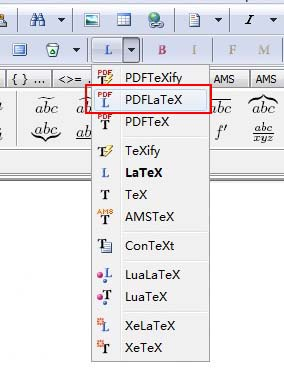
\includegraphics[width = 5cm]{latexSum/pdflatex.jpg}
\caption{不同编译选项选择方式}
\label{fig:pdflatex}
\end{figure}

排版时, 一般应尽量避免通栏图片的出现, 以节约版面. 
但通栏图并不少见. 通栏图一般应置于页面的顶端或底端. 
表~\ref{tab:insertFigFull} 中的代码将通栏图片插入页面底端的示例. 一般来说, 
以其会将底端通栏图片插入到“当前正文”所在页的\textbf{下一页面}底端. 

\begin{table}[!p]
\centering\footnotesize
\caption{通栏图置于页面底端代码示例}
\label{tab:insertFigFull}
\begin{tabular*}{7.9cm}{c@{\ }l}
\toprule[0.75pt]
1. & \textbackslash begin\{figure*\}[!b]\\
2. & \ \ \ \textbackslash centering \textbackslash small \\
3. & \ \ \ \textbackslash includegraphics[width = 16.4cm]\{figureSample.eps\}\\
4. & \ \ \ \textbackslash caption\{(图题、图注)\} \\
5. & \ \ \ \textbackslash label\{fig:table\} \\
5. & \textbackslash end\{figure*\}\\
\bottomrule[0.75pt]
\end{tabular*}
\end{table}

\section{表格}

期刊中所有的表格为“三线表”: 表中只有水平方向线条, 基本无垂直及倾斜线条
(如表~\ref{tab:1stPage}, \ref{tab:example}, 及 \ref{tab:example1}). 

排版人员应当了解表格设计的基本规范, 在排版时尽量修改. 表~\ref{tab:example} 为一典型的表格, 其体现的规范为

1.~列标题(表格最上方一行)应为具有“单位 (Unit)”的数值名称;

2.~表的第一列(纵向)常为不同方法(Meth)的列举;

3.~同一方法、不同条件(Condition)的结果, 在表格的横向方向排布. 相应的, 在表格的第二行, 
利用 \textbackslash cmidrule[0.5pt]\{$n$-$m$\} 语句绘制间断的水平线, 区分不同实验结果; 

4.~表格内容的进一步解释, 可以置于表的最下方. 
此时, 使用 \textbackslash multicolumn 命令设置表格多列合并可能导致表格
外观变化, 建议使用 minipage 的方法(具体见源文件).

\begin{table}[thp]
\footnotesize
\centering
\caption{Table example 1}
\label{tab:example}
\begin{tabular*}{7.9cm}{@{\extracolsep{\fill}}c@{}c@{}c@{}c@{}c@{}}
	\toprule[0.75pt]
	  \multirow{2}{*}{Meth}   & \multicolumn{2}{c}{Value 1 (Unit 1)} &   \multicolumn{2}{c}{Value 2 (Unit 2)} \\
\cmidrule[0.5pt]{2-3}\cmidrule[0.5pt]{4-5}
                   & Condition 1 & Condition 2& Condition 1 & Condition 2\\
	\midrule[0.5pt]
	   A     &    126    & 42.7 (1.6) &                    \phantom{1}8.2     &\phantom{1}9.5                 \\
	   B     &    175    & 42.9 (2.2) &                     11.1    & 10.5                 \\
	   C     &    176    & 44.1 (1.8) &                     11.3    & 15.5                 \\
	   D     &    148    & 40.0 (2.8) &                     27.1    & 30.5                 \\
	\bottomrule[0.75pt]
\end{tabular*}
	\begin{minipage}[c]{7.9cm}
    \vspace{2.5pt}
\scriptsize Supplementary information is listed here $\ldots$
\end{minipage}
\end{table}

\noindent 表~\ref{tab:example} 的具体代码可见 tex 源文件, 表格代码说明: 

1.~利用 tabular* 环境, 固定表格宽度 7.9~cm; 

2.~在设置列格式时, 
使用 @\{\textbackslash extracolsep\{\textbackslash fill\}\} 命令使各列在水平方向均匀分布, 
利用 @\{\} 清除各列间的间距, 压缩表格宽度; 


3.~使用~\textbackslash multirow 命令合并竖直方向的单元格;

4.~使用~\textbackslash multicolumn 命令合并水平方向的单元格;

5.~使用~\textbackslash phantom 命令生成伪字符, 保证数据在小数点位置处对齐. 

当表格内容相对简单时, 采用不固定表格宽度的方法, 
也可排出各列均匀分布的表格, 效果不错, 如表~\ref{tab:example1} 所示. 
其列格式设计要较表~\ref{tab:example} 更简单, 排版更快捷. 
通栏表格置底端的设置方法同图片(表~\ref{tab:insertFigFull}). 

\begin{table}[!b]
	\footnotesize
	\centering
	\caption{Table example 2}
	\label{tab:example1}
	\begin{tabular}{cccc}
		\toprule[0.75pt]
		Condition & Value 1 (m) & Value 2 (s) & Value 3 (kg)\\
		\midrule[0.5pt]
		126    & 42.7 (1.6) &   \phantom{1}8.2    &\phantom{1}9.5  \\
		175    & 42.9 (2.2) &             11.1    & 10.5           \\
		176    & 44.1 (1.8) &             11.3    & 15.5           \\
		148    & 40.0 (2.8) &             27.1    & 30.5           \\
		\bottomrule[0.75pt]
		\multicolumn{4}{l}{\scriptsize Additional information is listed here $\ldots$}
	\end{tabular}
\end{table}

\begin{table}[!b]
	\footnotesize
	\centering
	\caption{Modified Table 2 in ZUSC-D-17-0714}
	\label{tab:example2-714M}
	\begin{tabular*}{7.9cm}{@{\extracolsep{\fill}}l@{}c@{}c@{}}
		\toprule[0.75pt]
		Sturcture & Unsupervised/Supervised & Accuracy\\
		\midrule[0.5pt]
		Minimal SNN                & Supervised  & 75.93\%  \\
		\  (Tavanaei and Maida,       & & \\
		\ 2015)                      & & \\
		Spiking RBM                & Supervised  & 89.00\%  \\
		\  (Merolla et al., 2011) & &\\
		Dendritic neurons          & Supervised  & 90.30\%  \\
		\ \ (Hussain et al., 2014)     & & \\
		MD-SNN                     & Supervised  & 90.44\%  \\
		\  (our method) & & \\
		\bottomrule[0.75pt]
	\end{tabular*}
\end{table}


表格排版的几点考虑: 

1.~尽量将通栏表格转为单栏表格. 例如 ZUSC-D-17-0714 中表~2(如 表~\ref{tab:example2-714M} 所示), 
作者原稿为通栏表格(表~\ref{tab:example2-714}). 
考虑到表格仅有三列, 于是采用了“多行”表格的方式, 
将其压缩为单栏, 节省版面;


\begin{table*}[thp]
\footnotesize
\centering
\caption{Original Table 2 in ZUSC-D-17-0714}
\label{tab:example2-714}
\addtolength{\tabcolsep}{-2pt}
\begin{tabular*}{13cm}{@{\extracolsep{\fill}}lcc@{}}
\toprule[0.75pt]
\multicolumn{1}{c}{Sturcture} & Unsupervised/Supervised & Accuracy\\
\midrule[0.5pt]
 Minimal SNN (Tavanaei and Maida, 2015)    & Supervised  & 75.93\%  \\
 Spiking RBM (Merolla et al., 2011)        & Supervised  & 89.00\%  \\
 Dendritic neurons (Hussain et al., 2014)  & Supervised  & 90.30\%  \\
 MD-SNN (our method)                       & Supervised  & 90.44\%  \\
\bottomrule[0.75pt]
\end{tabular*}
\end{table*}

2.~必要时可缩写表头名称, 压缩表格宽度. 此时应注意在表格下方插入缩写词的全称. 


\section{数学公式}

\LaTeX{} 输出的数学公式形式优美, 是 \LaTeX{} 的关键优势. 
在 WinEdt 中, 由于有数学公式编辑界面的辅助(图~\ref{fig:ui}), 
数学公式的输入基本已实现了可视化. 排版人员应当大致阅读稿件, 
区分各符号是标量(白斜体)还是矢量(粗斜体), 在初排时尽量
更正公式中符号的字体. 

编辑部提供的 \LaTeX{} 模板中包含的
三个公式示例, 基本概括了常见的公式输入命令: 
\begin{equation}
\frac{\mathrm{d}}{\mathrm{d}t} {| \bar{\bm{x}}_{f_i} \cdot {\bm{W}}_{f_i}^l |^2 }= ({{\bm{W}}_{f_i}^l})^\mathrm{T} \dot {\bm{W}}_{f_i}^l \bar {\bm{x}}_{f_i} ({\bar {\bm{x}}_{f_i}})^\mathrm{T},
\end{equation}
\begin{equation}\label{indicatorfunc}
I_{j_1, j_2, \ldots, j_n}^{l_1, l_2, \ldots, l_n} (\bm{x}(t))=
	\begin{cases}
		\alpha(\bm{x}(t)), & \mathrm{if}\ \bm{x}(t) \in \Omega_{j_1, j_2, \ldots, j_n}^{l_1, l_2, \ldots, l_n}, \\
		0,                 & \mathrm{otherwise},
	\end{cases}
\end{equation}
\begin{equation}\label{eqn:Lyapdisturb1}
\begin{aligned}
	\dot{V} & \leq  - \lambda_{\min} ( K ) \| \bm{\xi} \|^2 - \lambda_{\min} ( K ) \| \bm{\zeta} \|^2                       \\
	        & \quad + \theta_\mathrm{ud} \| \bm{\xi} \| + 4 \rho \| \bm{\xi} \|^2                                           \\
	        & \leq  - \left[ ( \lambda_{\min} ( K )- 4 \rho ) \| \bm{\xi} \|  -  \theta_\mathrm{ud}  \right] \| \bm{\xi} \| \\
	        & \quad -\lambda_{\min} ( K ) \left\| \bm{\zeta} \right\|^2                                                     \\
	        & \leq 0.
\end{aligned}
\end{equation}

\section{参考文献}

进行 \LaTeX{} 写作、排版时, 通常使用 BibTeX 程序管理参考文献. 
作者投稿时, 将提供 .bib 格式的参考文献数据文件. 
生成排版所需的参考文献条目的步骤为: 

1.~首先编译 .tex 文件, \LaTeX{} 系统将
文稿中的所有交叉引用命令写入到 .aux 文件; 

2.~运行 BibTeX 程序(单击图~\ref{fig:ui} 中的 BibTeX 按钮), 其将依据新生成的 .aux 文件和稿件末尾的两行代码: 

\textbackslash bibliographystyle\{fitee\} \% 使用参考文献规范文件 fitee.bst

\textbackslash bibliography\{bibsample\}  \% 处理参考文献数据文件 bibsample.bib

生成符合 fitee 规范的 .bbl 文件(该文件将与 .tex 文件同名); 

3.~在编译 .tex 文件, 系统调用新生成的 .bbl 和 .aux 两文件, 插入交叉引用关系和参考文献条目; 

4.~修改 .bbl 文件内容, 使其满足期刊要求; 

5.~.tex 或 .bbl 文件编译出错时, 可能导致生成的 .aux 文件含有错误, 影响下一次编译的正确运行. 
此时, 应删除错误生成的 .aux 文件, 再编译 .tex 文件. 

实际初排时, .bbl 文件往往已经生成, 排版人员无需再运行 BibTex 程序, 
只需对 .bbl 文件修改即可. 
排版人员应注意, 一旦已对 .bbl 文件进行过修改, 就注意对其备份. 因为
WinEdt 的 \LaTeX{} 按钮与 BibTeX 按钮相邻, 极易误操作, 导致新修改的 .bbl 文件
被 BibTeX 覆盖. 

\begin{figure*}
\begin{equation}
\label{eqn:navi}
\rho\left(\frac{\partial \bm u}{\partial t} + \bm u \cdot \nabla \bm u\right)
= \rho \bm f
- \nabla p + \mu\nabla^2\bm u + (\mu+\mu^\prime)\nabla(\nabla\cdot \bm u).
\end{equation}
\end{figure*}


由于期刊采用作者-年代的引用形式, 排版人员应关注参考文献的引用的两种命令方式: 
\textbackslash cite\{$\cdot$\} 和 \textbackslash citep\{$\cdot$\}. 
当参考文献的引用在正文中起到句子成分的作用时, 使用 \textbackslash cite\{\} 命令; 
当参考文献的引用不起句子成分作用, 仅为补充用时, 使用 \textbackslash citep\{\} 命令. 
例如: 

1.~使用 \textbackslash cite\{\} 命令: Krause and Singer (2004) investigated the robust margin
loss of SVM that ceased to increase the penalty after a certain point.

2.~使用 \textbackslash citep\{\} 命令: 
The robust margin loss of SVM ceases to increase
the penalty after a certain point (Krause and Singer, 2004).




\section{杂项总结}

1.~注意左引号的输入方法 `abc', ``ABC''(参考代码)

2.~公式中括号的大小: 使用
\textbackslash big ($\times1.5$), 
\textbackslash Big ($\times2$),
\textbackslash bigg ($\times2.5$), 及
\textbackslash Bigg ($\times3$). 例如: 
\begin{equation*}
y = \Bigg(\bigg(\Big(\big(a(b+c) + d\big) + e\Big) + f\bigg) + g\Bigg) ,
\end{equation*}
与 \textbackslash left 和 \textbackslash right 的控制方式相比, 这类括号大小固定, 适用于公式换行的情形. 

3.~正体希腊字母: 使用 upgreek 宏包, 如 \textbackslash upalpha 输出为 $\upalpha$, \textbackslash uppi 输出为 $\uppi$

4.~不含章节编号的章节标题: \textbackslash section*\{title\}

5.~附录公式编号方法: 例如附录 A 中的公式编号设置方法如下: 

\noindent{\small \textbackslash setcounter\{equation\}\{0\}}

\noindent
{\small\textbackslash renewcommand\{\textbackslash theequation\}\{A\textbackslash arabic\{equation\}\}}

\noindent 附录中图、表及算法序号的设置方法, 同理. 


6.~特殊符号的输入: 

网页链接中, 符号‘\symbol{'176}’的输入: \textbackslash symbol\{'176\}
(此时使用符号‘\~{}’(\textbackslash\~{}\{\})链接无效); 
下划线的输入: \textbackslash \_

7.~软换行: 换行处加入 \textbackslash linebreak, 形如 MS-Word 中的 shift + enter

8.~插入 .jpg 图片: 利用 graphicx 宏包, 
使用 \textbackslash includegraphics[width=5cm]\{xxxx.jpg\}
的命令, 可以插入 .jpg 格式的图片, 其中, x 与 y 分别为图片的横、纵向像素数
插入图片的分辨率单位应为 dpi, 否则图片显示区域会出问题. 

9.~通栏公式的排版: 一个方案是利用通栏图片的环境, 
插入公式代码, 如本页的公式 (\ref{eqn:navi}). 

10.~稿件末页通常是不满页的, 需要平衡左右两栏的文字行数, 
使两栏的文字在底端对齐. 此时, 可以在参考文献部分之前, 插入
\textbackslash balance 命令, 自动设置两栏对齐. 
该命令通常是有效的, 但有时会造成稿件的段间距增大, 
版面不美观. 此时, 往往需要排版人员手动调整. 


%\balance
%\bibliographystyle{fitee}
%\bibliography{bibsample}

\begin{thebibliography}{}\footnotesize
	\itemsep -4pt
	\vspace{-8pt}
	
	\bibitem[\protect\astroncite{胡伟}{2011}]{Hu2011}
	胡伟, 2011.
	\newblock \LaTeX{} 2$\varepsilon$ 完全学习手册.
	\newblock 清华大学出版社, 北京.
	
	\bibitem[\protect\astroncite{刘海洋}{2013}]{Liu2013}
	刘海洋, 2013.
	\newblock \LaTeX{} 入门.
	\newblock 电子工业出版社, 北京.
	
	
\end{thebibliography}


\end{CJK}
\end{document}
